\heading{Introduction}
This lab focuses on configuring static IP addressing in a network comprising 6 PCs, 3 switches, and 3 serially connected routers. Static IP addressing is a fundamental networking concept where IP addresses are manually assigned to devices, ensuring consistent communication within the network. This setup is ideal for small, stable networks where device addresses do not change frequently.


\heading{Objectives}
\begin{enumerate}
   \item To configure static IP addresses on all PCs and router interfaces.
   \item To establish connectivity between all devices using static routing.
   \item To verify network functionality by testing communication between PCs across routers.
\end{enumerate}


\heading{Model}
\begin{figure}[th]
   \centering
   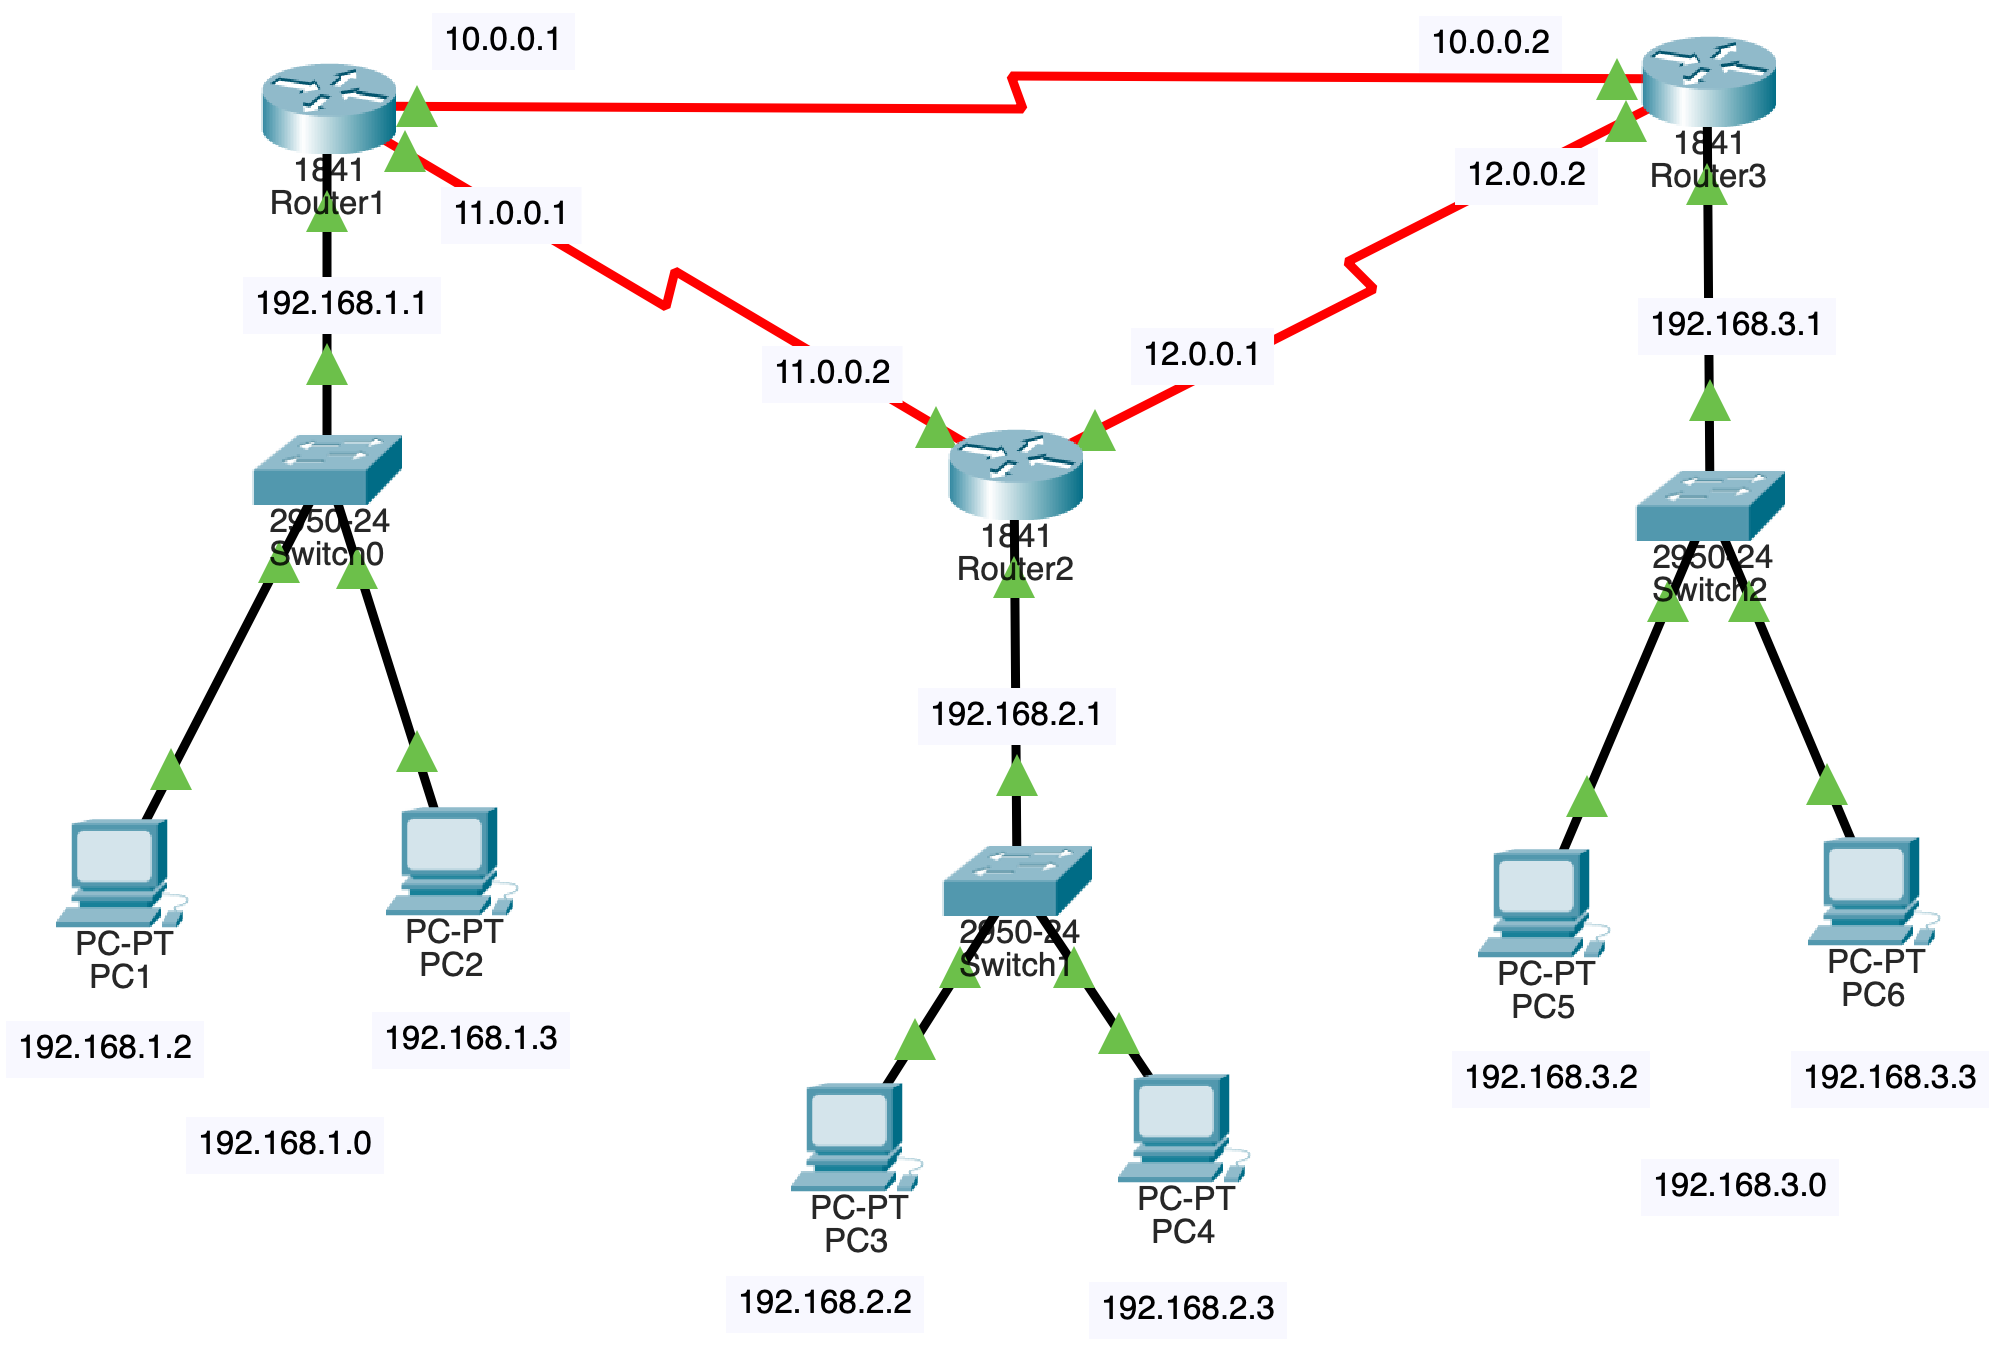
\includegraphics[width=0.8\textwidth]{figures/Exp-2.png}
   \caption{Static IP addressing with 6 PCs, 3 switches, and 3 serially connected routers.}
\end{figure}

\textbf{Model Description}
The network model consists of the following components:
\begin{enumerate}[itemsep=1ex]
   \item \textbf{Routers:} Three routers are used to interconnect different network segments. Each router is configured with static IP addresses on its interfaces to facilitate communication between subnets.
   \item \textbf{Switches:} Three switches are employed to connect PCs within the same subnet. Switches operate at Layer 2 and forward data based on MAC addresses.
   \item \textbf{Personal Computer (PC):} Six PCs are connected to the switches, each assigned a static IP address within their respective subnets. These PCs simulate end-user devices that require network access.
\end{enumerate}


\pagebreak
\heading{Routing Table}
\begin{tabularx}{\textwidth}{XXXX}
\textbf{Device Name} & \textbf{IP Address} &
\textbf{Subnet Mask} & \textbf{Default Gateway}\\
   PC1 & 192.168.1.2 & 255.255.255.0 & 192.168.1.1\\
   PC2 & 192.168.1.3 & 255.255.255.0 & 192.168.1.1\\
   PC3 & 192.168.2.2 & 255.255.255.0 & 192.168.2.1\\
   PC4 & 192.168.2.3 & 255.255.255.0 & 192.168.2.1\\
   PC5 & 192.168.3.2 & 255.255.255.0 & 192.168.3.1\\
   PC6 & 192.168.3.3 & 255.255.255.0 & 192.168.3.1\\
   
   Router1 (s/0/0) & 11.0.0.1 & 255.0.0.0\\
   Router2 (s/0/0) & 11.0.0.2 & 255.0.0.0\\
   
   Router2 (s/0/1) & 12.0.0.1 & 255.0.0.0\\
   Router3 (s/0/0) & 12.0.0.2 & 255.0.0.0\\

   Router1 (s/0/1) & 10.0.0.1 & 255.0.0.0\\
   Router3 (s/0/1) & 10.0.0.2 & 255.0.0.0\\
\end{tabularx}

\heading{Pinging Devices \& TTL}
\begin{figure}[th]
   \centering
   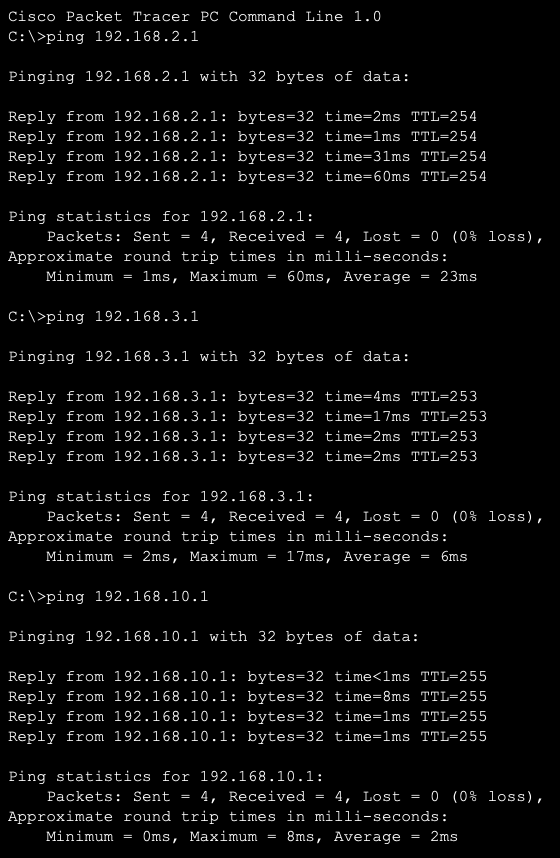
\includegraphics[width=0.5\textwidth]{figures/Exp-2-Ping.png}
   \caption{Pinging other devices from 192.168.1.2}
\end{figure}

\pagebreak
\heading{Complexity}
The network setup involves multiple subnets and requires careful planning of IP addressing schemes to avoid conflicts. Configuring static routes on the routers adds complexity, as each router must be manually programmed with the correct paths to ensure end-to-end connectivity. Additionally, verifying connectivity between all PCs requires thorough testing to ensure the configuration is error-free.

\heading{Discussion}
The lab successfully demonstrated the configuration of static IP addressing and static routing in a multi-router, multi-switch network. All PCs were able to communicate across subnets, confirming the correct implementation of static routes and IP addressing. This exercise highlighted the importance of meticulous planning and configuration in static network setups, particularly in ensuring seamless communication between devices.